\documentclass[11pt, a4paper]{article}

\usepackage{listings}
\usepackage{subfigure}
\usepackage{graphicx}
\usepackage{titling}
\usepackage[margin=1.8cm, includefoot]{geometry}
\usepackage{parskip}
\setlength{\parindent}{0cm}
\usepackage{titlesec}
\titlespacing\section{0pt}{6pt plus 2pt minus 2pt}{0pt plus 0pt minus 2pt}
\titlespacing\subsection{0pt}{4pt plus 2pt minus 2pt}{0pt plus 0pt minus 2pt}
\newcommand{\subtitle}[1]{
  \posttitle{
    \par\end{center}
    \begin{center}\large#1\end{center}
    \vskip0.5em}
}

\setlength{\droptitle}{-4em}

\begin{document}

\title{Deeva}
\subtitle{Quality Assurance Report}
\author{Kritaphat Sonsri-in, Xueqi Chen, Hector Dearman, \\Alina Draganescu, Felix de Souza}

\maketitle

Deeva\footnote{The story archtype used for this report is `The Quest' see and `The Hero with a Thousand Faces' \tt{https://speakerdeck.com/bipuldeb/seven-deadly-tricks-seven-ways-to-storytelling}} is a simple, non-magic Java debugger for teaching. It's unique selling point is that it will be able to graphically display the state of the Java program. It is built as a Java backend and Angular.js frontend stitched together with Python and Flask. Our supervisor is Dr Tristan Allwood.

\section{The Call}
The most interesting thing we read about QA was written by a software engineer working in the testing team at IBM which said that we should knowingly ship code with defects because ``unless we are NASA [...] customers want 99\% perfect code now, rather than 100\% working code in another five years at five times the price''\footnote{\tt{http://www.qntm.org/core }} and made a profound point that ``Software without testing is still valuable. Tests without software are worthless''\footnote{\tt{http://www.qntm.org/test }}. He then went on to write: ``Robust testing separates the adults from the children. It separates software on which we can build a business from software we can't give away.'' 

As programmers we want to write software that's correct, reliable, fast and secure; software that's perfect. QA techniques can help improve the quality of our projects but, equally importantly, they let us measure how good our software is so we can calibrate the level of quality to meet the goals of the project owners\footnote{Gary Bernhardt talks about this as ``maintaining the correct level of ass'' \tt{http://www.confreaks.com/videos/615-cascadiaruby2011-the-unix-chainsaw}}. So with that in mind we look at how we are managing the quality of our project. 

\section{The Journey}
Initially, working on autopilot, we implemented unit tests, system tests and set up a continuous integration server. 


Then we had a meeting with Tristan. 


He pointed out several things that we hadn't thought about, things that would make a better product. For example, a sketch of the layout and design of the user interface would be helpful to avoid ``This week we have to demo this feature'' UX design; a usage scenario which should contain the basic run through of each feature in the project. Also problems like how we integrate the program with lab machines; how it should handle broken user input elegantly; how we should support different resolutions of the screens in college. We also discussed the types of quality specifically of our project such as correctness, performance, reliability and security. Our meeting really helped get us thinking about how we could apply QA techniques to our project specifically.
\section{Types of Quality}	
\subsection{Correctness}
A debugger is useless (and thus causes more harm than good) if it alters the usual behaviour of the program being invasively debugged. It can introduce Heisenbugs\footnote{\tt{http://en.wikipedia.org/wiki/Heisenbug}}, that make the debugging process even more difficult. To mitigate this, we're using the Java Debug Interface (JDI) library which in turn launches the code to be debugged in a separate Java Virtual Machine (JVM). We then create requests to do debug actions and also listen out for when these events happen. Leveraging the JDI means we're already building on software that has been rigorously tested and as a result should reduce any possibility of Heisenbugs.

One of our requirements was for Deeva to be `simple'. Although not to be misinterpreted as lacking functionality, our ideal would be for the user to be able to quickly build a good mental model of the reaction of the program to any input - the Principle of Least Surprise\footnote{\tt{http://www.faqs.org/docs/artu/ch11s01.html}}. This principle is interesting because it allows us to save time reinventing the wheel, however it could also inhibit a much needed change which would only make the user experience better. Great importance is thus placed on the User Interface (UI) (which should get out of the way\footnote{\tt{http://www.cooper.com/journal/2012/08/the-best-interface-is-no-interface}}) as we want users to be able to pick up and use the debugger without much effort, however we don't want to `inherit' the same caveats other debuggers may have. Striking that balance is what we're currently in the midst of doing. 

In order to evaluate the usability of our debugger, we must turn to the target audience, as developers aren't necessarily a good measure to go by when testing a UI they created. This is due in part to the fact that we have a much more accurate mental model. Provided we stick to our schedule and have a minimal but working demo by week 7, we are planning on having first-year students (our target audience) test our debugger and get usability feedback from them.

Drawing from Valve's `Sound Practices of Games, Business and Design\footnote{\tt{http://www.valvesoftware.com/publications/2005/AGDC2005\_SoundPractices.pdf}}' we're going to try and apply the following techniques as part of our user testing procedure:
\begin{itemize}
\item Having a minimal set of documentation (and on-screen cues) and asking fewer questions allows the user to make an exploratory approach to using our program, giving us really important feedback. We hope to achieve this by taking a more task-oriented approach i.e. give them a task to do rather than offer up leading questions. If combined together with filming the user, we may also pick up on things that the user may not even say in their structured and well-thought out response (involuntary responses, acclimitisation problems etc.).
\item Getting the user to provide a running commentary whilst they use the program allows us to capture the user's first (and candid) responses, which will provide greater insight to usability of the debugger.
\item Another tool was (as developers) to not say anything, which really just enforces the first point, as we want to ascertain how usable our app is without the help of a nearby developer.
\end{itemize}

\subsection{Performance}
For Deeva we're interested in a couple of types of performance:
\subsubsection{Startup time}
This is the time it takes Deeva to get from hitting enter on the command line to being able to accept user input. This is important because tools that are slow to start are painful to use and hence are used less\footnote{It's not a direct parallel but if we consider websites, page abandonment approaches 50\% as load time reaches about 10 seconds see: \tt{http://blog.kissmetrics.com/loading-time/?wide=1}}. You can only improve what you measure so we wrote a script that iterates over the git history, starts Deeva and times how long until it's accepting the first request \footnote{We got the idea for doing this from Gary Bernhardt screencast: \newline
 \tt{https://www.destroyallsoftware.com/screencasts/catalog/time-to-first-request}}. We can then display the results using a custom D3 graph (see Figure \ref{fig:figure1}).
 
\begin{figure}[h]
\centering
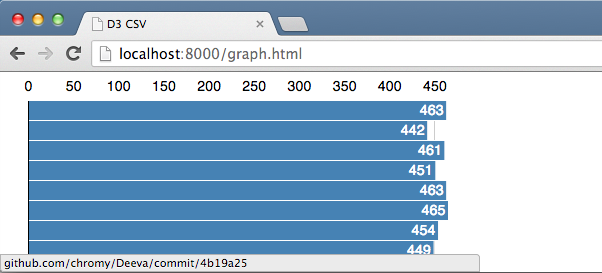
\includegraphics[height = 45mm]{testing.png}
\caption{Development Practices}
\label{fig:figure1}
\end{figure} 
 
As you can see our app currently takes roughly 450ms to load. If we see that one commit increased the time-to-first-request, we can click on it and it will take us to the relevant commit on github so we can work out what went wrong. We also added a test to fail if Deeva takes over a second to start.
\subsubsection{Responsiveness}

Similarly to startup time the responsiveness of a tool is a large contributing factor to how nice it is to use (and for similar reasons). An article from Nielsen Norman\footnote{\tt{ http://www.nngroup.com/articles/response-times-3-important-limits/}} divides responses into three categories: under 100ms, 100ms to 1s and 1s to 10s. 

Less than 100 milliseconds is imperceptible: you feel like you are manipulating the data directly. From 100ms to 1 second: a delay is noticeable but it doesn't interrupt your thoughts. 1 to 10 seconds is the dead zone where you would want to do something else\footnote{ It helped our intuition to consider how often we would run test suites which took 100ms, 1s and 10s.}. Ideally we want to respond in under 100ms and failing that, in under a second. This is difficult to measure and ultimately we decided the cost of automating it wasn't worth it over a such short and fixed time schedule, instead we could use Chrome's built in tools to identify slow REST endpoints if and when it became a problem in user testing. This isn't ideal but the best we could do in the circumstances.

\subsubsection{Performance Hit}
Another factor that affects debuggers is the performance of the program being debugged. Fortunately for us this is not a big issue, this debugger is for teaching and is spec'd for toy examples rather than enterprise Java, while it would be nice to have a debugger with a low performance measure it's not worth the cost to measure in this case.
\subsection{Reliability}
It's easy to lose sight of the fact that debuggers necessarily take broken programs as input. Thus it is imperative that our debugger does not crash whilst also trying to debug a buggy program (which we can consider as malformed input). Thus we need plenty of good examples of broken code, code that will try to break our debugger and thus test the robustness of our code.
\subsection{Security}
In terms of security, we are much less at risk when compared to a web service (even though we are using web technologies) as the debugger is running locally on the machine and the only data we have is the users program. Considering our target audience (first year computing students) most code will be contrived examples not consisting of sensitive data.

Considering a wider target audience, there are still some risks as a result of how we're building the debugger and how we expect it to be used (through a web browser interface). Some of these risks should be mitigated by a strong network policy but we should try to minimise these risks. These risks include:
\begin{itemize}
\item A remote connection to the web server that serves up the debugger interface to the user. We can defend against this and a resulting session hijack by displaying a link containing a secret key that can only be seen if the person connecting was the same person starting the web server instance. This (together with session management and a strong network policy) should also defend against an attempt to get at any sensitive data the user may have.
\item We also don't want to introduce a problem of simultaneous connections (even if the secret key is known) as that could display inconsistent states to both connections. To mitigate this, we can try and enforce one connection at a time.
\end{itemize}
However in general, security is not a big QA concen with us compared to the other factors aforementioned.
			
\section{Arrival and Frustration}

So now we know specifically what problems we face but how do we solve them? Below we've gone through in detail the techniques we have used and plan to use to deliver the software. 
\subsection{Development practices}
\subsubsection{Usage Scenarios}
	
\begin{figure}[h]
\centering
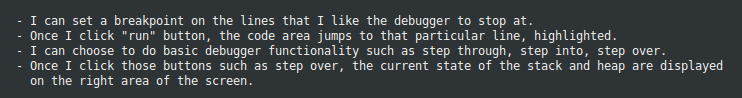
\includegraphics[width = 160mm]{usage.png}
\caption{Usage Scenarios}
\label{fig:figure6}
\end{figure} 	
	
A usage scenario is a script which we can run through that hits each feature in our program and is a demonstration of using the program to solve a simple problem (see Figure \ref{fig:figure6}).

\subsubsection{Unit Tests}
	
\begin{figure}[h]
\centering
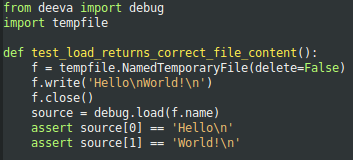
\includegraphics[height =40mm, width = 85 mm]{unit_test.png}
\caption{Unit Test}
\label{fig:figure5}
\end{figure} 	
	
An essential part of testing is the unit tests, it give us minute-to-minute confidence that code is still correct when we change the code, especially after a massive refactor. We are using multiple languages, which each have their own unit testing framework i.e. QUnit for JavaScript, JUnit for Java and nose for Python (see Figure \ref{fig:figure5}).

\subsubsection{System Tests}
As our user interface is through the web browser, we use Lettuce (a Python port of the Ruby BDD tool Cucumber) which drives Selenium which drives a browser (see Figure \ref{fig:figure2}). 

\subsubsection{BDD and TDD}
We believe that some form of test driven development results in better quality code but as relative newcomers to test driven development it is really hard to remember to write tests up front, especially as on the new project lots of what we write is explorative\footnote{Try and convince somebody they should spike some horrible piece of Java integration they finally got working.}. However we're trying really hard to move to a ``write failing feature test $\rightarrow$ write failing unit test $\rightarrow$ write code $\rightarrow$ make unit test pass $\rightarrow$ make feature test pass'' double loop methodology.
\subsubsection{Continuous Integration}
We use Travis CI as a continuous integration server. This gives us confidence that all the tests pass in a completely fresh environment and more importantly emails us when somebody breaks something so we can fix it.

\begin{figure}[h]
\centering
\subfigure[Lettuce System Test]{%
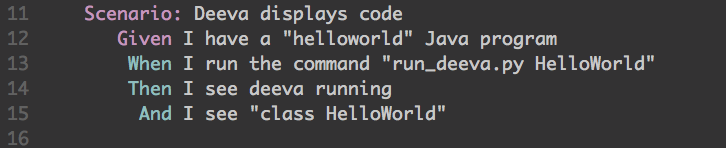
\includegraphics[width=85mm, height=23mm]{test2.png}
\label{fig:figure2}}
\quad
\centering
\subfigure[Travis Build]{%
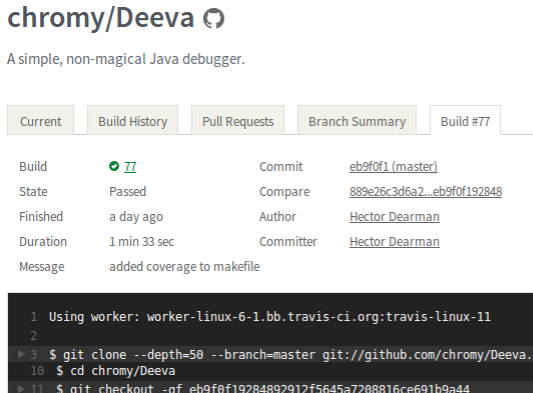
\includegraphics[height=60mm]{travis2.png}
\label{fig:figure3}}
\caption{Development Practices}
\label{fig:figure4}
\end{figure}
  
\subsubsection{Version Control}
We use git hosted on Github for source control. We decided against having a production and staging branch, which make sense in large projects but not so much considering the complexity and scope of our project. As an alternative, we opted to use the lower complexity approach using git tag to tag stable versions. 

We considered using a code review tool such as Gerrit, but we decided it was too heavy-weight and the initial overhead wasn't worth it. If any of us were significantly worried, we would use our Trello board to move the story card into ``In Review'' which someone could address, or we would address at our next meeting. We decided to go with a lower complexity approach again, where we would merge code ourselves, preferably testing before committing i.e. accepting social responsibility versus enforcement via tools. Should a broken build occur (notified via Travis), we all stop and try to address the issue.
\subsubsection{Pair programming}

Pair programming improves efficiency and quality. When we code in pairs the rate of defects introduced is lowered. Some teams pair program all the time, we decided to do pair programming in labs when we are working on a high complexity story (normally a story with story points 8 or above). The reason we decided to not fully embrace pair programming is out of concern for our velocity\footnote{Currently, out velocity is 12 story points/week and we are currently one week behind. In order to finish our product by the end of week 9 of term we estimate that we need to increase our velocity to 15 story points/weeks.}, which is not at our ideal at the moment. The effect of pair programming is difficult to measure, anecdotally the benefits usually outweigh or equal the overhead\footnote{\tt{http://opinionateddevelopment.blogspot.co.uk/2011/04/programming-velocity-connundrum.html}} involved but we have multiple constraints that a typical work environment doesn't such as different work schedules and various other commitments. 

\section{The Final Ordeal (Guaranteeing Quality)}


It is not enough to just to pay lip service to QA. Like justice it needs to be done and seen to be done. It's all very well telling the project owner that ``we're following best practices to produce good software'' but they only care about results: ``What guarantees can you give me about Deeva?''. We responded (jokingly) with ``It will probably turn up.'' We negotiated from there to come up with a couple of useful tests we would use to guarantee the quality of our project.

We decided to guarantee the quality of Deeva using the following techniques: 
\begin{itemize}
\item
Using metrics like test coverage\footnote{ We can use plugins for our testing tools like nose-coverage and the Python project \tt{https://pypi.python.org/pypi/mccabe to get these statistics.
}}, cyclomatic complexity and doc coverage to show that code quality is good for future maintainers.
\item
Demoing usage scenarios, if we can walk through a full scenario then we can demonstrate that most features work as Tristan intended.
\item
The Acid test: sitting a student down with Deeva and buggy program and see if they can fix it without prompting which is the ultimate test of whether Deeva works. 

\end{itemize}

\section{The Goal}

It's easy to just hack on the code (and we might have been able to get away with it even on this project) but hacking doesn't scale. Projects eventually become too big for even the cleverest person to fit in their head all at once. The cost of adding a feature or fixing a bug goes up and up until eventually the project sputters and dies\footnote{ Dr Robert Chatley - Software Engineering Design (220) 2012}.

So it's easy just hack away but if we ever want programmers to be taken seriously as engineers then it starts on the first day of every project when we put into place the methodologies and techniques that will allow us to deliver fast, correct, reliable and secure software on time, on budget and on spec.

And we're not there yet. ``But it does not matter how slowly you go so long as you do not stop''\footnote{Confucius 479 BC}.


\end{document}
